\documentclass[a4paper,12pt]{article}
\usepackage[utf8]{inputenc}
\usepackage{ae}
\usepackage{pslatex}
\usepackage[portuges]{babel}
\usepackage{indentfirst}
\usepackage[portuguese,noprefix]{nomencl}
\usepackage{setspace}
\usepackage[colorlinks,allcolors=black]{hyperref}
\usepackage{enumitem}
\usepackage[ampersand]{easylist}
\usepackage{fancyhdr}
\usepackage{graphicx}

\setlength{\oddsidemargin}{2.5cm}
\setlength{\evensidemargin}{2.5cm}
\setlength{\textwidth}{15cm}
\addtolength{\oddsidemargin}{-1in}
\addtolength{\evensidemargin}{-1in}
\setlength{\topmargin}{2.0cm}
\setlength{\headheight}{1.0cm}
\setlength{\headsep}{1.0cm}
\setlength{\textheight}{22.7cm}
\setlength{\footskip}{1.0cm}
\addtolength{\topmargin}{-1in}
\singlespacing

\begin{document}
\begin{titlepage}
\begin{center}
\centering
\linespread{2.0}
\Huge\Huge\textbf{M1} \\
\huge\huge\textbf{Projeto de modelagem} \\
\LARGE\LARGE\textbf{Sistema de gerenciamento de votos} \\
\vfill
\end{center}
\textbf{Discente: } Ailson Forte dos Santos \\
\textbf{Disciplina: } DIM0504 - Análise de Projeto Orientado a Objetos (APOO) \\
{\par\hfill\today}
\end{titlepage}
\newpage
\tableofcontents

\newpage
\section*{Descrição da aplicação}
\markright{}
\addcontentsline{toc}{section}{Descrição da aplicação}
Desde os tempos mais antigos a humanidade busca conhecer os padrões existentes no mundo. Uma das ferramentas que criamos para esse fim foi a coleta e análise de dados. Os primeiros censos demográficos que se tem notícia foram elaborados pelos chineses e romanos e eram executados por militares e fiscais. O mais antigo é datado de 2238 a.C. realizado na China pelo imperador Yao com o objetivo de coletar informações sobre o número de pessoas e lavouras cultivadas.
\par Dentre as formas de realização de censo, destacamos as pesquisas de opinião, com o intuito de mostrar a realização da democracia. Elas nos mostram como está a satisfação de um determinado grupo de individuos, ou seja, um país, estado, pessoas de uma mesma religião, etc; com relação ao assunto abordado pela pesquisa.
\par Desenvolveremos nesse projeto um sitema que visa gerenciar essas pesquisas. Nosso intuito é, através de enquetes e eleições, falitar a coleta desses dados. Seja para propósitos simples como a cor favorita de determinado grupo de indivíduos ou algo mais complexo como a eleição para presidente de um país. Nela, o usuário poderá criar e gerenciar sua própria pesquisa ou eleição.

\newpage
\section*{Requisitos}
\markright{}
\addcontentsline{toc}{section}{Requisitos}
\subsection*{Regras gerais deste sistema:}
\markright{}
\addcontentsline{toc}{subsection}{Regras gerais deste sistema}

\begin{easylist}[itemize]
& O sistema possui eleitores e juizes de eleição.
& As enquetes/eleições só devem ser cadastradas por juízes de eleição.
& Qualquer usuário não cadastrado é eleitor. Eleitores e juízes de eleição podem votar livremente de acordo com as regras estabelecidas pelo juiz criador da enquete/eleição.
& Juízes de eleição não podem modificar votos, apenas validá-los.
& Todo voto é secreto e direto, ou seja, apenas juízes podem ver quem votou e divulgar o resultado da votação de suas próprias enquetes/eleições.
\end{easylist}

\newpage
\section*{Casos de uso}
\markright{}
\addcontentsline{toc}{section}{Casos de uso}
\subsection*{Diagrama de casos de uso}
\markright{}
\addcontentsline{toc}{subsection}{Diagrama de casos de uso}
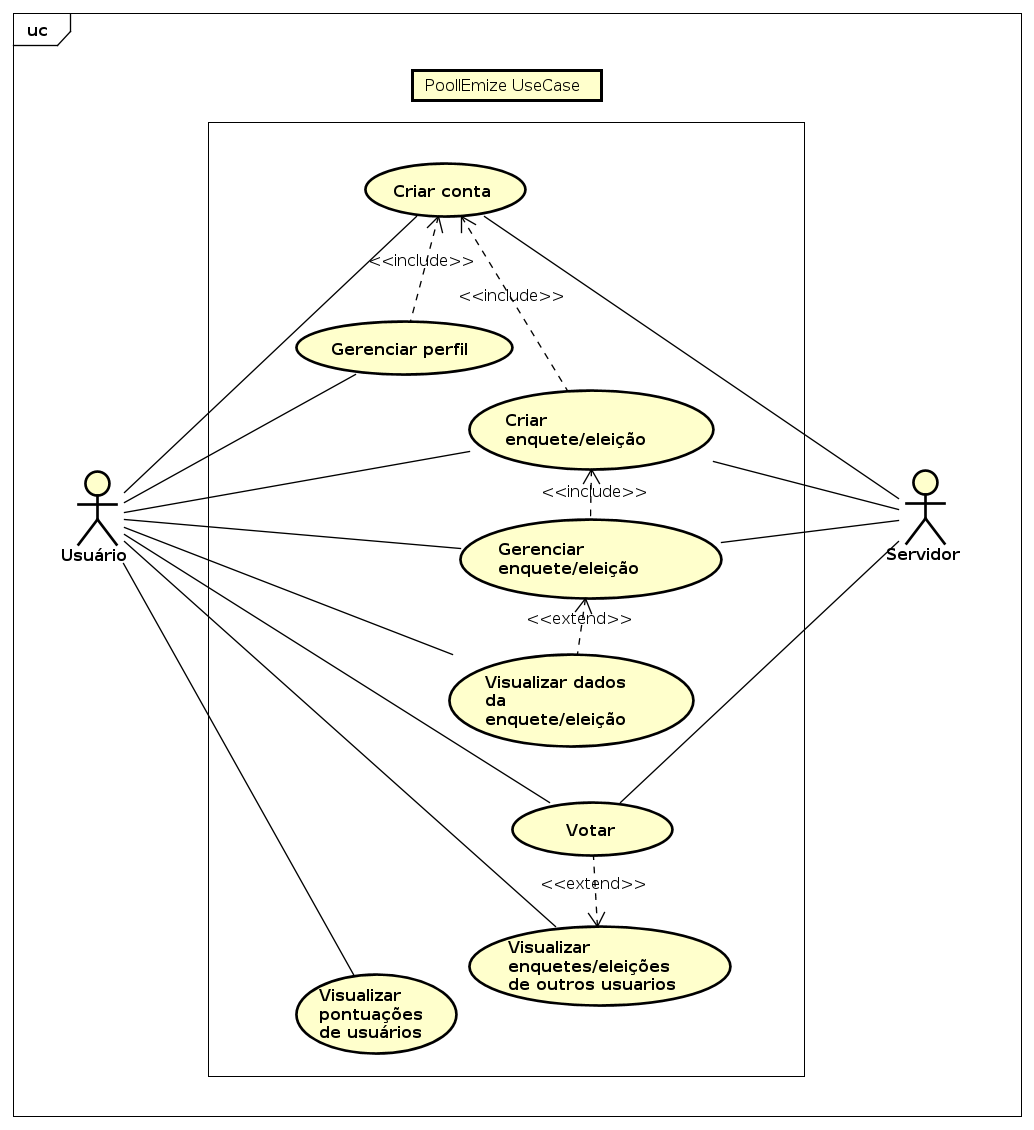
\includegraphics[width=15cm]{use_cases/UseCaseDiagram0.png}
\par
\subsection*{Descrição dos casos de uso}
\markright{}
\addcontentsline{toc}{subsection}{Descrição dos casos de uso}

\begin{center}
{\subsubsection*{Criar Conta (CSU01)}}
\end{center}
\markright{}
\addcontentsline{toc}{subsubsection}{Criar Conta (CSU01)}
\begin{tabular}{|c|}\hline
	{\textbf{Ator principal:}} Usuário \\
	{\textbf{Atores secundários:}} Sistema\\
	\hline
\end{tabular}

\newpage
\section*{Referências}
\markright{}
\addcontentsline{toc}{section}{Referências}
\par\url{https://www.aedb.br/seget/arquivos/artigos13/28518220.pdf}
\par\url{https://en.wikipedia.org/wiki/Census}
\par\url{https://en.wikipedia.org/wiki/Demography}



\end{document}